\documentclass[11pt, oneside]{article} 
\usepackage{geometry}
\geometry{letterpaper} 
\usepackage{graphicx}
	
\usepackage{amssymb}
\usepackage{amsmath}
\usepackage{parskip}
\usepackage{color}
\usepackage{hyperref}

\graphicspath{{/Users/telliott_admin/Dropbox/Tex/png/}}
% \begin{center} 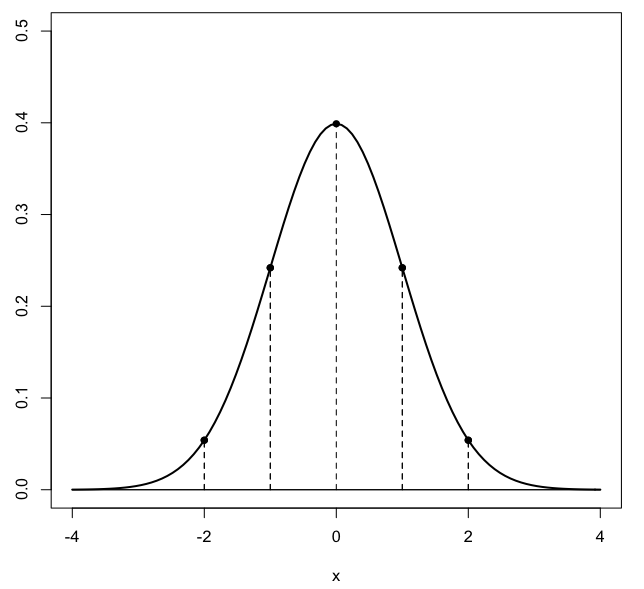
\includegraphics [scale=0.4] {gauss3.png} \end{center}

\title{Derivation of Taylor Series}
\date{}

\begin{document}
\maketitle
\Large
\subsection*{first}
We consider a function $f$ that is analytic inside and on the circle $C_0:  z = r_0$, centered at $0$.  The point $z$ is interior to $C_0$ and the Cauchy integral formula applies ($w$ is on $C_0$):
\[ f(z) = \frac{1}{2 \pi i} \ \int_{C_0} \frac{f(w) \ dw}{w - z} \]

The factor $1/(w-z)$ can be rewritten as
\[ \frac{1}{w - z} = \frac{1}{w} \cdot \frac{1}{1 - (z/w)} \]

\subsection*{aside on the geometric series}
We recall that the nth partial sum of the geometric series can be written
\[ S_N = \sum_{n=0}^{N-1} z^n = 1 + z + z^2 \dots + z^{N-1} \]
(starting our numbering with the 0th term, the last term is $N-1$).

So
\[ z \ S_N = \sum_{n=0}^{N-1} z^n = z + z^2 \dots + z^{N} \]
\[ (1-z) \ S_N = 1 - z^N \]
\[ S_N = \frac{1 - z^{N}}{1 - z} \]
\[ S_N = \frac{1}{1-z} - \frac{z^{N}}{1 - z} \]
so finally
\[ \frac{1}{1 - z} = \sum_{n=0}^{N-1} z^n +  \frac{z^{N}}{1 - z} \]

\subsection*{return to the problem}
We had
\[ \frac{1}{w - z} = \frac{1}{w} \cdot \frac{1}{1 - (z/w)} \]
\[ = \frac{1}{w} \cdot \ [ \  \sum_{n=0}^{N-1} (z/w)^n +  \frac{(z/w)^{N}}{1 - z/w} \ ] \]
\[ = \sum_{n=0}^{N-1} \frac{1}{w^{n+1}} z^n +  \frac{z^{N}}{w^{N-1}(w - z)} \]

Multiply through by $f(w)$ and then integrate:
\[ \int_C \frac{f(w)}{w - z} \ dw  = \sum_{n=0}^{N-1} \int_C \frac{f(w) \ dw}{w^{n+1}} z^n +  z^{N} \int_C \frac{f(w) \ dw}{w^{N-1}(w - z)} \]
The left-hand side is $2 \pi i f(z)$.

Recall that (around $z = 0$) we had as an extension of the Cauchy Integral theorem:
\[ f^n(0) = \frac{n!}{2 \pi i} \int_C \frac{f(w)}{w^{n+1}} \ dw \]

Hence the first term on the right-hand side in the previous expression is
\[ \frac{2 \pi i}{n!} \sum_{n=0}^{N-1} f^n(0) \ z^n \]
They show that the second term on the right-hand side is the remainder that will go to zero as $N \rightarrow \infty$, so (after dividing by $2 \pi i$, we obtain  
\[ f(z) = \lim_{N \rightarrow \infty} \frac{1}{n!} \sum_{n=0}^{N} f^n(0) \ z^n + \]


\end{document}